\section{Cyclic decomposition, quarter-turn, and oriented Catalan moment}
\label{iii:sec:catalan}

The dodecaphase record relates the constitutive response to
other transport invariants. The link is established on determined subspaces
and maps: the rank defect measures an incidence difference,
the determinant preserves a scalar response, and a coefficient
of the resolvent retains orientation. The collection of moments culminating
in Catalan's constant enters at this last level.

\subsection{Two subspaces of the dodecaphase cycle}

In $\mathbb R^{12}$, let $C e_j=e_{j+1\bmod12}$ and let
\begin{equation}
 P_3^{\mathrm{cyc}}=\frac{I+C^3+C^6+C^9}{4},\qquad
 P_4^{\mathrm{cyc}}=\frac{I+C^4+C^8}{3},\qquad
 H_d=\operatorname{Ran}P_d^{\mathrm{cyc}}.
 \label{iii:eq:projectors34}
\end{equation}
The averages over cyclic subgroups are orthogonal projectors.
$H_3$ consists of the periodic sequences whose period divides $3$,
and $H_4$ of those whose period divides $4$. Their dimensions are $3$ and $4$.
The restriction of $C$ to each space realizes the corresponding cycle.
The superscript $\mathrm{cyc}$ identifies the average over the dodecaphase cycle:
$P_3^{\mathrm{cyc}}$ is the projector onto sequences whose period divides
$3$. Its domain and action differ from those of the three-dimensional
isotypic projector of the icosahedral realization; equality of rank
does not identify the two operators.

\begin{proposition}[Rank defect and determinantal response]
The following identities hold:
\begin{equation}
 \frac{\operatorname{Tr}(P_3^{\mathrm{cyc}}-P_4^{\mathrm{cyc}})}{12}=-\frac1{12},\qquad
 \frac{\det_{H_3}(I-sC)}{\det_{H_4}(I-sC)}
 =\frac{1-s^3}{1-s^4}=f(s),\quad 0<s<1.
 \label{iii:eq:trace-det}
\end{equation}
\end{proposition}
\begin{proof}
The trace of an orthogonal projector is its rank, so the numerator
of the first expression is $3-4$. The characteristic polynomial of a cycle
of length $d$ is $t^d-1$; hence its determinant $\det(I-sC)$ is
$1-s^d$. Their quotient yields the second identity.
\end{proof}

The substitution $s=q^{30}$ transports this representation to the
$90/120$ quotient. At $s=1$, the common constant mode is cancelled before taking
the limit, which equals $3/4$. This realization of $-1/12$ as a trace defect
has an explicit finite domain. The regularized and modular
realizations of the same scalar retain their own operators and domains.

\subsection{Faithful representation of the quarter-turn}

Define the antipodal projector $P_{\rm ant}=(I-C^6)/2$ and
$Q=P_4^{\mathrm{cyc}}P_{\rm ant}$. This projector acts on the twelve-phase cycle and
differs from the constitutive projector $P_-$ in Section~\ref{iii:sec:constitutiva}.
The projectors $P_4^{\mathrm{cyc}}$ and $P_{\rm ant}$ commute, and
$Q$ has rank $2$. In its image, fix the orthonormal basis
\begin{equation}
 u=\frac1{\sqrt6}(1,0,-1,0,1,0,-1,0,1,0,-1,0)^{\mathsf T},
 \qquad v=Cu.
 \label{iii:eq:uv}
\end{equation}
Componentwise verification gives $Cu=v$ and $Cv=-u$. Consequently,
the isometry $W(a,b)=au+bv$ satisfies
\begin{equation}
 CW=WJ,\qquad
 J=\begin{pmatrix}0&-1\\1&0\end{pmatrix},\qquad J^2=-I.
 \label{iii:eq:quarter-intertwiner}
\end{equation}
The complex structure of the plane is realized by the effective action of
the cycle. The sign depends on the chosen orientation: in the same basis,
$C^3W=-WJ$. This precision allows the plane to be composed with the oriented readout.

\subsection{Resolvent and unlimited depth}

Since $C^2=-I$ on $\operatorname{Ran}Q$, for $0\leq s<1$ one has
\begin{equation}
 (I-sC)^{-1}\big|_{\operatorname{Ran}Q}=\frac{I+sC}{1+s^2},
 \qquad k_4(s):=\langle v,(I-sC)^{-1}u\rangle=\frac{s}{1+s^2}.
 \label{iii:eq:resolvent}
\end{equation}
The sequence $\langle v,C^nu\rangle$ is $0,1,0,-1,\ldots$. The depth
readout preserves this character through the moment
\begin{equation}
 \mathcal C_2(s)=\sum_{k\geq0}\frac{(-1)^ks^{2k+1}}{(2k+1)^2},
 \qquad 0\leq s\leq1.
 \label{iii:eq:c2}
\end{equation}
The series converges absolutely and uniformly on this interval by
comparison with $\sum(2k+1)^{-2}$. For $0<s<1$, the differentiated series
converge uniformly on every compact subinterval of the interior. With
$\mathcal D=s\,d/ds$, one obtains
\begin{equation}
 \mathcal D^2\mathcal C_2(s)=k_4(s),\qquad
 \mathcal C_2(s)=\int_0^s\frac{dt}{t}\int_0^t\frac{d\xi}{\xi}\,k_4(\xi).
 \label{iii:eq:c2-integral}
\end{equation}
The conditions $\mathcal C_2(0)=0$ and
$\lim_{s\downarrow0}\mathcal D\mathcal C_2(s)=0$ fix the two integration
constants. Indeed, the difference between two solutions of
$\mathcal D^2F=k_4$ has the form $a\log s+b$; the second condition
annuls $a$ and the first annuls $b$.
Uniform convergence permits evaluation at the endpoint $s=1$: the result is
the Catalan moment. The finite representation of the character preserves its
orientation; the depth index remains unlimited.

\subsection{Composition with the constitutive response}

\begin{theorem}[Constitutive differential relation]
For $0<s<1$, with the orientation of \eqref{iii:eq:uv},
\begin{equation}
 f(s)=\frac{1+s+s^2}{s(1+s)}\,\mathcal D^2\mathcal C_2(s).
 \label{iii:eq:catalan-vacuum}
\end{equation}
\end{theorem}
\begin{proof}
Substituting \eqref{iii:eq:resolvent} into \eqref{iii:eq:c2-integral} and using
$(1+s)(1+s^2)=1+s+s^2+s^3$ gives the identity. All denominators are
positive on the domain. The intertwiner \eqref{iii:eq:quarter-intertwiner}
identifies the operator coefficient used before its evaluation.
\end{proof}

Upon evaluating $s_\pm=q_\pm^{30}$, the same collection produces the two channel
responses of \eqref{iii:eq:rchannels}. The Catalan limit, the trace
defect, and the constitutive eigenvalues retain their distinct functions
within this composition. Reversing the cycle with the markings $u,v$
fixed changes the sign of $k_4$ and preserves the determinant $1+s^2$.
This identifies orientation information that the determinant
alone does not distinguish.

The Pell development uses a particular evaluation of this collection,
with $\rho=2-\sqrt3$ and $\rho^{-1}=2+\sqrt3$. Its proof is retained as
a distinct unit of integration; the angular definition of $q_\pm$ remains
independent of any eventual identification of $s_\pm$ with $\rho$.

Figure~\ref{iii:fig:respuesta-momento-pell} represents the relation between
the rational response and the oriented kernel before integration. The Pell
section satisfies $\rho+\rho^{-1}=4$, so that
$k_4(\rho)=(\rho+\rho^{-1})^{-1}=1/4$. The two constitutive values
are obtained, by contrast, by evaluating $f$ at the already constructed
arguments $s_\pm$. The plot includes the continuous extensions of the two
functions to $[0,1]$; the domain of constitutive inversion remains
the open interval $(0,1)$.

\begin{figure}[htbp]
\centering
\begin{tikzpicture}[x=10cm,y=4.6cm,>=stealth]
 \pgfmathsetmacro{\pellrho}{2-sqrt(3)}
 \pgfmathsetmacro{\fpell}{(1+\pellrho+\pellrho^2)/(1+\pellrho+\pellrho^2+\pellrho^3)}
 \draw[gray!35,thin] (0,0.25)--(1,0.25);
 \draw[gray!35,thin] (0,0.5)--(1,0.5);
 \draw[gray!35,thin] (0,0.75)--(1,0.75);
 \draw[gray!35,thin] (0,1)--(1,1);
 \draw[->] (0,0)--(1.04,0) node[right] {$s$};
 \draw[->] (0,0)--(0,1.1) node[above] {dimensionless value};
 \foreach \xx/\lab in {0/0,0.5/{1/2},1/1}{
  \draw (\xx,0)--(\xx,-0.015) node[below] {$\lab$};
 }
 \foreach \yy/\lab in {0.25/{1/4},0.5/{1/2},0.75/{3/4},1/1}{
  \draw (0,\yy)--(-0.008,\yy) node[left] {$\lab$};
 }
 \draw[gray!70,densely dashed] (\pellrho,0)--(\pellrho,1.035);
 \node[below,align=center,font=\small] at (\pellrho,-0.015)
  {$\rho$\\[-1pt]$2-\sqrt3$};
 \draw[black,very thick,domain=0:1,samples=121,smooth]
  plot (\x,{(1+\x+\x^2)/(1+\x+\x^2+\x^3)});
 \draw[blue!65!black,thick,dashed,domain=0:1,samples=121,smooth]
  plot (\x,{\x/(1+\x^2)});
 \fill[black] (\pellrho,\fpell) circle[radius=1.7pt];
 \fill[blue!65!black] (\pellrho,0.25) circle[radius=1.7pt];
 \node[anchor=south west,font=\small,fill=white,inner sep=2pt] at (0.51,0.94)
  {$f(s)=\dfrac{1+s+s^2}{1+s+s^2+s^3}$};
 \node[anchor=south west,text=blue!65!black,font=\small] at (0.57,0.55)
  {$k_4(s)=\dfrac{s}{1+s^2}$};
 \node[anchor=north west,font=\small,fill=white,inner sep=2pt]
  at (0.30,0.225) {$k_4(\rho)=1/4$};
\end{tikzpicture}
\caption{Constitutive response and kernel of the oriented moment. The solid
curve is $f$ and the dashed curve is
$k_4=\mathcal D^2\mathcal C_2$; they are related by
\eqref{iii:eq:catalan-vacuum}. The vertical line marks the Pell section,
without identifying it with the constitutive arguments $s_+$ or $s_-$.}
\label{iii:fig:respuesta-momento-pell}
\end{figure}
